%!TEX root = main.tex

\section{Motivation}

\begin{frame}{Motivation}{Why do we care?}
    \begin{itemize}
        \item password cracking has an inherent parallel structure
        \item FPGAs enable to exploit true parallelism
    \end{itemize}
    \begin{itemize}
        \item bcrypt claims to resists hardware optimisations
        \item implementation presented last year\footnote{\tiny \url{http://www.openwall.com/presentations/Passwords13-Energy-Efficient-Cracking/}} can be optimized
    \end{itemize}
    \begin{itemize}
        \item play with expensive hardware
    \end{itemize}
\end{frame}
\note{\begin{itemize}
\item OpenWall bcrypt implementation on different platforms: \begin{itemize}
\item (mainly) parallela/epiphany board
\item zedboard
\item Xeon Phi
\item Haswell\end{itemize}
\item Problems with FPGA implementation: \begin{itemize}
\item only implemented cost loop in fabric
\item wait cycles
\item 14 cores with very unbalanced resource utilization\end{itemize}
\end{itemize}}

\section{FPGAs}

\begin{frame}[plain]
    \center
    \vspace{-10mm}
    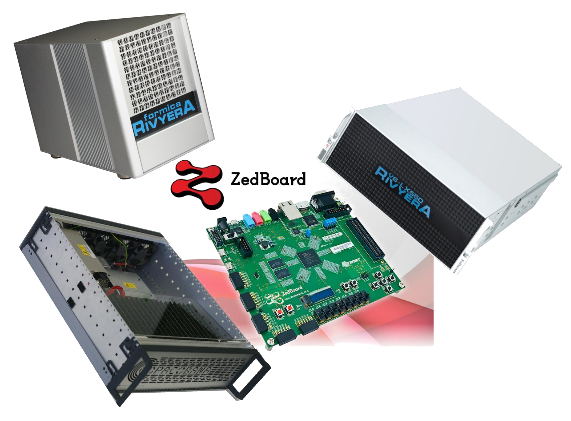
\includegraphics[height=\textheight]{data/fpgas.png}
\end{frame}
\note{
What are FPGAs?
\begin{itemize}
\item[short:] (re-)programmable hardware
\item[long:] see next slides
\end{itemize}}

\begin{frame}{What are FPGAs?}{GPCPUs $\leftrightarrow$ FPGAs $\leftrightarrow$ ASICs}
    \visible<1->
    Field Programmable Gate Arrays lie between General Purpose CPUs and Application Specific Integrated Circuits. They combine advantages from both.
    \begin{columns}[T]
      \begin{column}{.45\textwidth}
        \visible<2->{
        \begin{exampleblock}{Advantages}
        \begin{itemize}
          \item fast to program
          \item low level hardware design
          \item re-programmable
        \end{itemize}
        \end{exampleblock}}
      \end{column}
      \begin{column}{.45\textwidth}
        \visible<3->{
        \begin{alertblock}{Drawbacks}
        \begin{itemize}
          \item slower clock speed
          \item lower resource utilization
        \end{itemize}
        \end{alertblock}}
      \end{column}
    \end{columns}
    \visible<4->{
    \vspace{5mm}
    In contrast to CPUs, parallelism is directly expressible, but one does not have to design everything down to transistor level.}
\end{frame}
\note{\begin{itemize}
\item CPUs have general functions
\item supports wide range of applications
\item[$\Rightarrow$] good in many points but not best in specific applications
\item ASICs require huge design effort
\item tedious modeling and simulation down to gate-level
\item[$\Rightarrow$] fastes hardware for specific applications
\item FPGAs easier to program than ASICS
\item re-programmable (loadable with task specific programs)
\item allow low level hardware design while still abstracts from gate level
\end{itemize}}

\begin{frame}{What are FPGAs?}{How does it work?}
  \begin{columns}[T]
    \begin{column}{.75\textwidth}
      FPGAs are build mainly out of
      \begin{itemize}
          \item Look Up Tables (LUTs)
          \item Flip Flops (FFs)
          \item Block RAMs (BRAMs)
          \item Digital Signal Processing units (DSPs)
      \end{itemize}
      but can contain hard instantiated cores\\(e.g.\, ARM Cortex A9, etc.)
    \end{column}
    \begin{column}{.25\textwidth}
    \vspace{-10mm}\hspace{-12mm}
    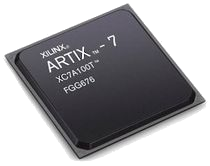
\includegraphics[height=25mm]{data/zynq.png}
    \end{column}
  \end{columns}
\end{frame}
\note{contains different kind of logic blocks \begin{itemize}
\item LUTs are needed for custom logic function
\item FFs to register LUT outputs, build local storage, reduce critical path, re-programmable routes
\item BRAMs bigger local storage, still accessible within one clock cycle
\item DSPs for signal processing (multiply accumulate)
\item other hard instantiated cores (e.g.\, ARM Cortex A9)
\end{itemize}}

\begin{frame}{What are FPGAs?}{Artix7}
    \center 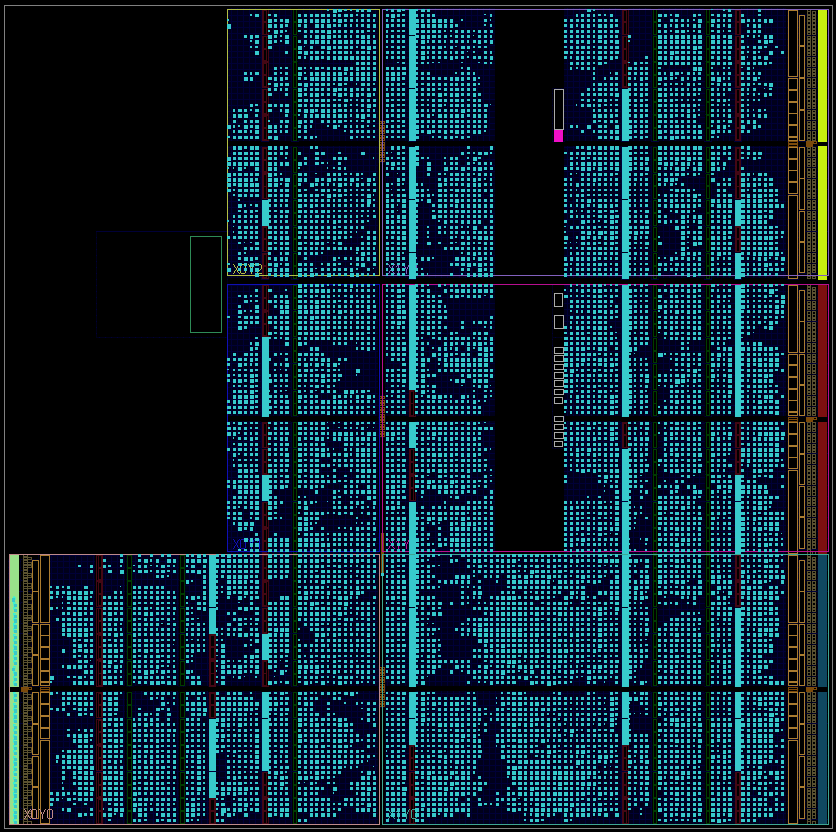
\includegraphics[height=.80\textheight]{data/artix7.png}
\end{frame}
\note{\begin{itemize}
\item Fabric is the place were all logic is located
\item BRAM and DSPs are arranged column wise
\item LUTs and FFs are arranged in slices\\(2 slices per configurable logic block (CLB))
\end{itemize}}

\begin{frame}{What are FPGAs}{Slice}
    \center
    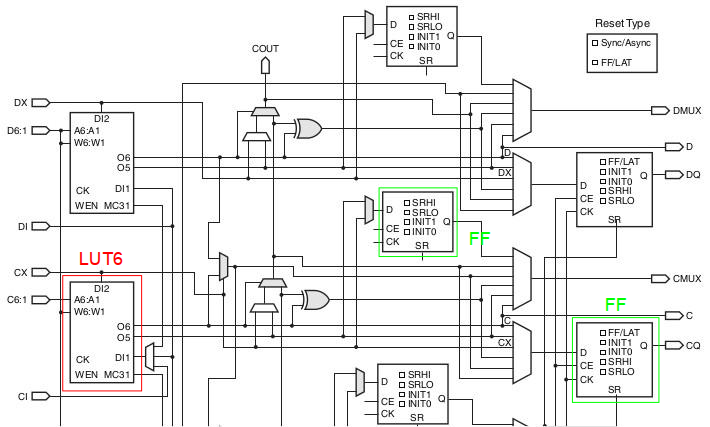
\includegraphics[width=.90\textwidth]{data/slice.png}

    {\footnotesize Xilinx 7 Series SliceM, c.f.\, UG474}
\end{frame}
\note{\begin{itemize}
\item 4 LUT6, 8 FFs per slice (2 FFs per LUT6)
\item additional muxer, fast carry path, etc.
\item[]
\item is this important to know?
\item well.. depends :-)
\item one has to know how the hardware is build up, to get best performance (respect the hardware)
\end{itemize}}

\begin{frame}{FPGA-Cluster}{}
    \visible<2->{
    \center 
\includegraphics[height=.80\textheight]{data/meme.jpg}}
\end{frame}
\note{What are FPGA Cluster? \begin{itemize}
\item similar to GPU cluster
\item aim: improve parallel performance
\end{itemize}}

\begin{frame}{FPGA-Cluster}{}
    \begin{columns}[T]
      \begin{column}{.45\textwidth}
        FPGA Cluster like \textsc{copacobana} or \textsc{rivyera} combine many FPGA chips.

        \vspace{5mm}\hspace{5mm}
        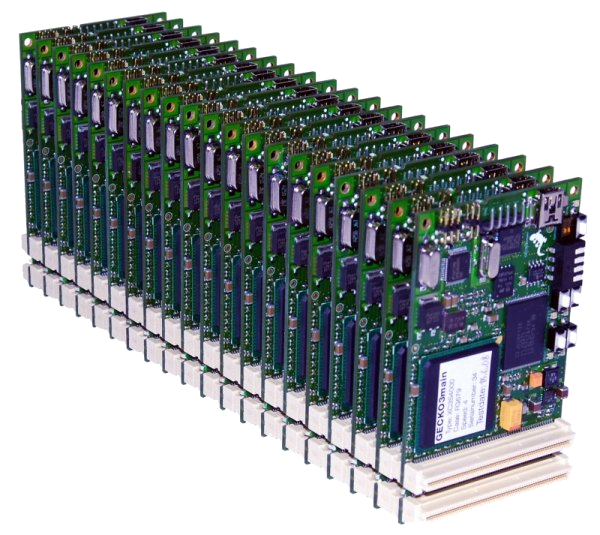
\includegraphics[height=.40\textheight]{data/fpga_cluster.png}
      \end{column}
      \begin{column}{.45\textwidth}
      \visible<2->{
       \begin{block}{Can we use this?}
        \begin{itemize}
          \item Yes!
          \item split password range between every FPGA
          \item with small overhead, this results in a nice speed up
        \end{itemize}
      \end{block}}
      \end{column}
    \end{columns}
\end{frame}
\note{\begin{itemize}
\item example for cluster:\begin{itemize}
\item \textsc{copacobana}\begin{itemize}
\item 120 low power Spartan3 FPGAs\end{itemize}
\item \textsc{rivyera}\begin{itemize}
\item 64 Spartan6 FPGAs\end{itemize}\end{itemize}
\item Why is this useful for us?\begin{itemize}
\item Password Range can be split up at synthesis time
\item every FPGA works independently
\item with few dependencies, this results in quasi linear speed up\end{itemize}
\end{itemize}}

\section{bcrypt}
\begin{frame}{What is bcrypt?}
    Introduced in 1999 by Provos and Mazi\`{e}res.\footnote{\tiny \url{http://www.usenix.org/events/usenix99/full_papers/provos/provos.pdf}}
    \begin{columns}[T]
    \visible<2->{
      \begin{column}{.45\textwidth}
       \begin{block}{EksBlowfish}
      \begin{itemize}
          \item block cipher based on blowfish
          \item expensive key schedule
          \item encryption equals blowfish encryption
      \end{itemize}
      \end{block}
      \end{column}}
    \visible<3->{
      \begin{column}{.45\textwidth}
       \begin{block}{bcrypt}
      \begin{itemize}
          \item cost-parameterized
          \item uses EksBlowfishSetup (key schedule) and encryption
      \end{itemize}
      \end{block}
      \end{column}}
    \end{columns}
    \visible<4->{
    \vspace{5mm}
    Implemented in OpenBSD 2.1, Ruby on Rails, PHP as standard password hash.}
\end{frame}
\note{\begin{itemize}
\item proposed two constructions
\item \emph{EksBlowfish} less known, but serves as underlying building block for bcrypt
\item itself is based on blowfish, expensive key schedule
\item \emph{bcrypt} cost parameterized hash function
\item cost factor controlls computational efford of \texttt{EksBlowfishSetup}
\item practical applications in OpenBSD, Ruby on Rails, PHP
\item We start with explaining the key schedule
\end{itemize}}

\begin{frame}{What is bcrypt?}{EksBlowfishSetup}
    \center
      \begin{block}{Pseudocode}
        \begin{algorithm2e}[H]
          \KwIn{cost, salt, key}
          \KwOut{state}
          $state \leftarrow$ InitState$()$\;
          $state \leftarrow$ ExpandKey$(state, salt, key)$\;
          \KwSty{Repeat} ($2^{cost}$) \Begin{
            $state \leftarrow$ ExpandKey$(state, 0, salt)$\;
            $state \leftarrow$ ExpandKey$(state, 0, key)$\;
          }
          \KwRet{$state$}\;
          \caption{EksBlowfishSetup}
        \end{algorithm2e}
      \end{block}
\end{frame}
\note{\begin{itemize}
\item state consists of 4 SBoxes, each 256 $\times$ \SI{32}{\bit} and
\item 18 \SI{32}{\bit} P-values (subkeys) $\Rightarrow$ \SI{4}{\kilo\byte} memory
\item initialized with digits of $\pi$
\item \texttt{ExpandKey} updates state (see next slide)
\item number of iterations exponential in cost parameter
\item $ExpandKey(state, 0, .)$ equals blowfish key schedule
\end{itemize}}

\begin{frame}{What is bcrypt?}{ExpandKey}
    \center
    \begin{block}{ExpandKey}
        Modified version of blowfish key schedule. XORes the key onto subkeys
        and afterwards, updates the state sequentially.\\
        Calls \texttt{bf\_enc} 521 times per invocation.
    \end{block}
    \begin{block}{State Update}
        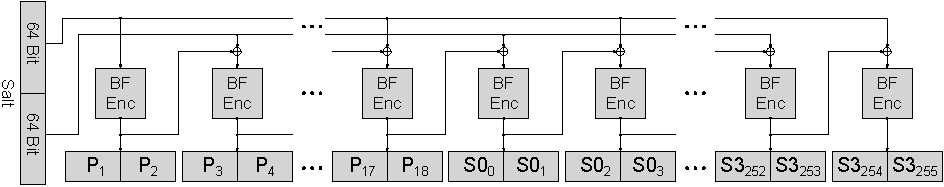
\includegraphics[width=\textwidth]{data/expandkey.pdf}
    \end{block}
\end{frame}
\note{\begin{itemize}
\item \texttt{ExpandKey} blowfish encrypts lower \SI{64}{\bit} of Salt
\item Result substitutes $P_1$, $P_2$ and
\item gets xored with higher \SI{64}{\bit} of Salt, encrypted again\ldots
\item Alltogether 521 blowfish encryptions per call
\item How does blowfish encryption works?
\end{itemize}}

\begin{frame}{What is bcrypt?}{blowfish encryption}
    \center 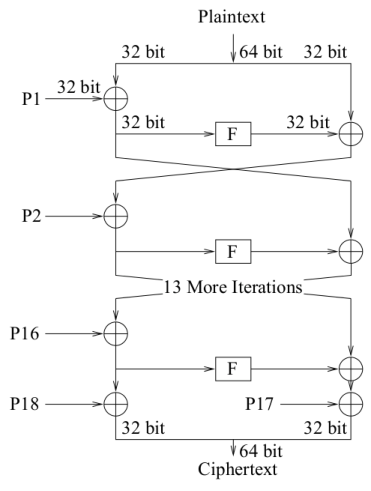
\includegraphics[height=.80\textheight]{data/blowfish.pdf}
\end{frame}
\note{\begin{itemize}
\item simple 16 round Feistel network
\item in every round: key xor, f-Function xor, swap
\item f-Function consists of 4 SBox look ups, 2 additions, 1 xor
\item finalize: xor $P_{17}$, $P_{18}$
\item \SI{64}{\bit} block size
\item[$\Rightarrow$] nice minimalistic structure
\end{itemize}}

\begin{frame}{What is bcrypt?}{bcrypt}
    \center
      \begin{block}{Pseudocode}
        \begin{algorithm2e}[H]
          \KwIn{cost, salt, key}
          \KwOut{hash}
          $state \leftarrow$ EksBlowfishSetup$(cost,salt,key)$\;
          $ctext \leftarrow$ ``OrpheanBeholderScryDoubt''\;
          \KwSty{Repeat} ($64$) \Begin{
            $ctext \leftarrow$ EncryptECB$(state, ctext)$\;
          }
          \KwRet{Concatenate$(cost,salt,key)$}\;
          \caption{bcrypt}
        \end{algorithm2e}
      \end{block}
\end{frame}
\note{\begin{itemize}
\item bcrypt itself is quite simple
\item calls \texttt{EksBlowfishSetup} followed by
\item 64 blowfish encryptions in ECB mode of  magic value (3 blocks)
\item[$\Rightarrow$] allmost all work/time is spent during key schedule
\end{itemize}}

\begin{frame}{Where are we?}
    \begin{block}{bcrypt is}
    \begin{itemize}
        \item based on blowfish
        \item cost-parameterized password hash
        \item sequential
    \end{itemize}
    \end{block}
    \visible<2->{
    \begin{block}{bcrypt needs}
    \begin{itemize}
        \item exponential (in \emph{cost}) loop iterations
        \item \SI{4}{\kilo\byte} memory
    \end{itemize}
    \end{block}}
\end{frame}
\note{\begin{itemize}
\item bcrypts cost depend only on many sequential blowfish encryption
\item authors claim randomly accessed memory is costly
\end{itemize}}

\section{Design of Cracker}
\begin{frame}{Design of Cracker}
    \center 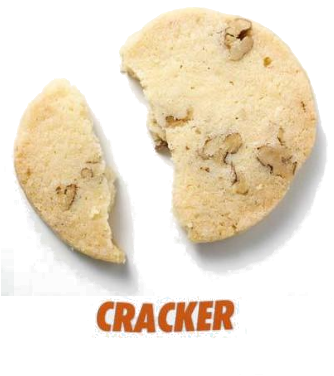
\includegraphics[height=75mm]{data/cracker.png}
\end{frame}
\note{\begin{itemize}
\item we have no chance to parallelize bcrypts structure
\item does the memory consumption hurt?
\item depends on target FPGAs
\end{itemize}}

\begin{frame}{Target Platforms}{zedboard}
    Low cost, low power FPGA
    \begin{columns}[T]
      \begin{column}{.5\textwidth}
       \begin{block}{Specs}
      \begin{itemize}
        \item Zynq-7000 XC7Z020 FPGA (comarable to Artix7)
        \item ARM Cortex A9 CPU
        \item HDMI, VGA, Ethernet, Audio, USB, JTAG, SD Card, Buttons\ldots
      \end{itemize}
      \end{block}
      \end{column}
      \begin{column}{.45\textwidth}
        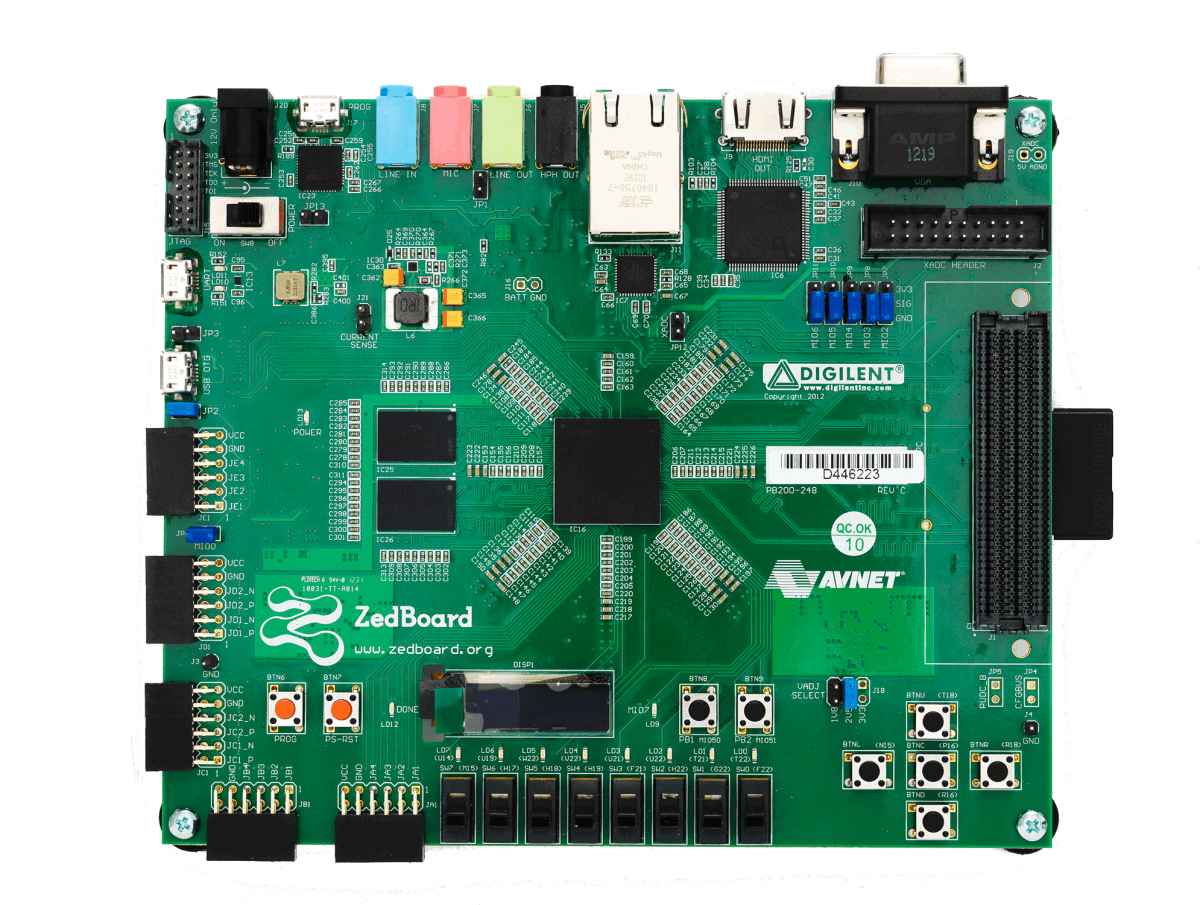
\includegraphics[width=\textwidth]{data/zedboard.png}
      \end{column}
    \end{columns}
\end{frame}
\note{\begin{itemize}
\item OpenWall project also targeted zedboard
\item combines ARM Cortex A9 with programmable logic
\item contains 140 \SI{18}{\kilo\bit} BRAMs
\item embedded Linux can be run from SD card
\end{itemize}}

\begin{frame}{Target Platforms}{\textsc{rivyera}}
    High Performance FPGA cluster
    \begin{columns}[T]
      \begin{column}{.5\textwidth}
       \begin{block}{Specs}
      \begin{itemize}
        \item 64 Spartan6 LX150\\(available with up to 128)
        \item i7 CPU
        \item 16 GB RAM
      \end{itemize}
      \end{block}
      \end{column}
      \begin{column}{.45\textwidth}
        \vspace{10mm}
        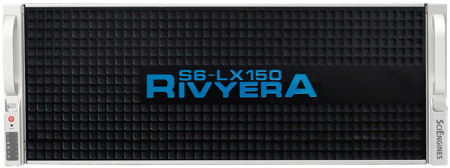
\includegraphics[width=\textwidth]{data/rivyera.png}
      \end{column}
    \end{columns}
    \vspace{5mm}
    Up to 10 \textsc{rivyera}s can be fit into a standard rack.
\end{frame}
\note{\begin{itemize}
\item \textsc{rivyera} is the actual FPGA cluster available @ EmSec
\item contains up to 128 Spartan6 (ours: 64)
\item each Spartan6 268 \SI{18}{\kilo\bit} BRAMs\\
      (roughly twice as big as Artix7 on zedboard, but slower speed grade)
\end{itemize}}

\begin{frame}{Optimization Goal}
    \center \Huge
    Low Area Footprint
\end{frame}
\note{
Design Goal?
\begin{itemize}
\item simple Feistel structure will allow high clock rates
\item[$\Rightarrow$] keep area footprint as low as possible
\item[$\Rightarrow$] fit as many cores onto on FPGA as possible
\end{itemize}}

\begin{frame}{Design of Cracker}
    \begin{block}{API}
      \begin{itemize}
          \item keep API minimalistic $\Rightarrow$ low bandwidth interface
          \item transfer target \emph{salt} and \emph{hash}
          \item start cracker
          \item on success, read \emph{password}
      \end{itemize}
    \end{block}
    \visible<2->{
    \begin{block}{Password Generation}
      \begin{itemize}
          \item on-chip password generation
          \item needs no bandwidth
          \item split password range at synthesis-time
      \end{itemize}
    \end{block}}
\end{frame}
\note{\begin{itemize}
\item
\end{itemize}}

\begin{frame}{Design of Cracker}
    \begin{block}{bcrypt Core}
      \begin{itemize}
          \item memory for SBoxes, subkeys, key and initial values
          \item almost no logic needed for algorithm
          \item consists mainly of BRAM look ups
      \end{itemize}
    \end{block}
    \visible<2->{
    \begin{alertblock}{Problematic}
      \begin{itemize}
          \item memory for password storage
          \item registers require to much logic
      \end{itemize}
    \end{alertblock}}
\end{frame}
\note{\begin{itemize}
\item 2 SBoxes per BRAM, subkeys in 1 extra Bram
\item initial values take another 2 BRAMs (can be shared)
\item but: how to store passwords?
\item registers in logic are to costly
\item[$\Rightarrow$] quad-core design
\end{itemize}}

\begin{frame}{Design of Cracker}
    \begin{block}{Quad Core}
      \begin{itemize}
          \item bundle four bcrypt cores together
          \item store four passwords in one BRAM
          \item during initialization, password generator can access BRAM
          \item core0, core1 and core2, core3 can access the BRAM alternately
      \end{itemize}
    \end{block}
    \visible<2->{
    \begin{exampleblock}{Advantages}
      \begin{itemize}
          \item cores need access only during begin of \texttt{ExpandKey}
          \item[] thus, they only diverge by 36 clock cycles
      \end{itemize}
    \end{exampleblock}}
\end{frame}
\note{\begin{itemize}
\item dual port BRAM allows 2 read/write accesses per clock
\item bundle 4 cores, alternate their memory access phases
\item password generator can access the memory during 256 initialization cycles
\item cores diverge only by 36 clock cycles
\end{itemize}}

\begin{frame}{Design of Cracker}{Resulting Design}
    \center 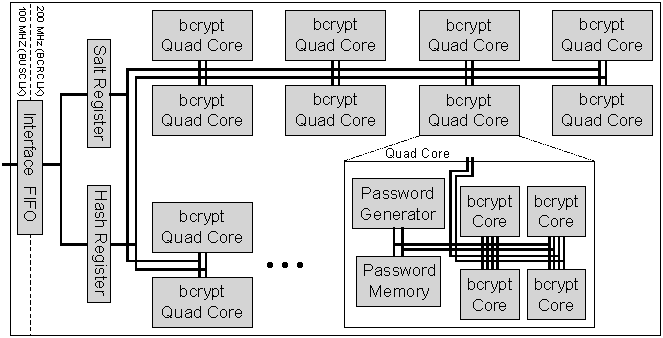
\includegraphics[width=.90\textwidth]{data/cracker_overview.pdf}
\end{frame}
\note{\begin{itemize}
\item every quad core operates fully independent on his own password subrange
\end{itemize}}

\begin{frame}{How to interface the Cracker?}
    Different possibilities for zedboard:
    \begin{itemize}
        \item AXI4 Interfaces \begin{itemize}
            \item[+] low area footprint
            \item[--] more complex to implement
            \end{itemize}
    \visible<2->{
        \item Xillybus \begin{itemize}
            \item[+] abstracts from AXI4 Interfaces
            \item[+] Linux support $\Rightarrow$ easy to demonstrate
            \item[--] proprietary
            \item[--] \enquote{fat}, i.e.\, higher resource consumption
            \end{itemize}}
    \end{itemize}
    \visible<3->{
    Custom interface for \textsc{rivyera} needed.}
\end{frame}
\note{}

\begin{frame}{How to interface the Cracker?}{}
    \begin{block}{Xillybus}
      \begin{itemize}
        \item stream access through FIFOs or DMA into fabric logic
        \item abstraction from AXI4 is quite nice
        \item Linux driver $\Rightarrow$ just write to \texttt{/dev/xillybus\_mem\_8}
      \end{itemize}
    \end{block}
    \visible<2->{
    \begin{block}{Memory Layout}
      \center 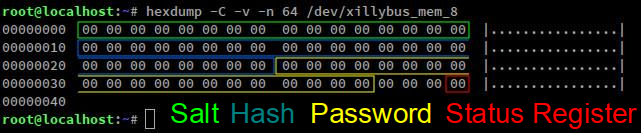
\includegraphics[width=\textwidth]{data/mem_layout.png}
    \end{block}}
\end{frame}
\note{\begin{itemize}
\item Linux driver allows DMA into logic
\item host side interface consists only of file write/reads.
\item Status Register:\begin{itemize}
\item low nibble used for host-to-FPGA communication (reset, start)
\item high nibble used for FPGA-to-host communication (done, success)\end{itemize}
\end{itemize}}

\begin{frame}{Design of Cracker}{Resulting Resources}
    \begin{block}{zedboard}
      \begin{itemize}
          \item estimations for one zedboard:
          \item[] 28 cores as upper bound, BRAMs as limiting resource
          \item first design attempt (password in registers):
          \item[] 12 cores fit, LUT utilization way to high
          \item Quad Core Design:
          \item[] 24 cores fit, with using \enquote{fat} interface
      \end{itemize}
    \end{block}
    \visible<2->{
    \begin{block}{\textsc{rivyera}}
      \begin{itemize}
          \item Quad Core Design:
          \item[] 48 cores per Spartan6 $\Rightarrow$ 3072 cores on whole \textsc{rivyera}
      \end{itemize}
    \end{block}}
\end{frame}
\note{\begin{itemize}
\item with Xillybus 24 cores @ \SI{200}{\mega\hertz} possible (zedboard)
\item with custom interface 48 cores @ \SI{100}{\mega\hertz} possible (\textsc{rivyera})
\end{itemize}}

\section{Demo}
\begin{frame}{Demo}
    \center 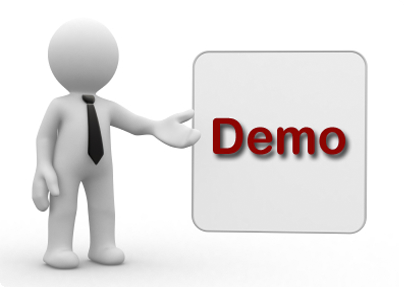
\includegraphics[height=50mm]{data/demo.png}
\end{frame}
\note{\begin{itemize}
\item demonstrate interface :-)
\end{itemize}}

\section{Results}
\begin{frame}{Results}{Compared to GPUs}
\begin{block}{cost Parameter and Hash-rates}
\begin{table}[tp]
  \centering
  \begin{tabular}{l r r r r}
    \toprule
              & \multicolumn{4}{c}{Target (CPU) runtime}\\
              &\quad 1ms \quad   &\quad 10ms \quad   &\quad  100ms \quad   &\quad  1000ms \quad   \\
    \midrule
    bcrypt cost    & 3.69   & 7.03    & 10.3      & 13.6   \\
    \midrule
                   & \multicolumn{4}{c}{Hashs per Second}\\
                   & \quad 1ms \quad & \quad 10ms \quad & \quad 100ms \quad & \quad 1000ms \quad\\
    \midrule
    {\bf zedboard} &{\bf 9,230 H/s}  &{\bf 916.25 H/s}  &{\bf 98.77 H/s}    &{\bf 9.93 H/s}     \\
    Spartan-6      &{9,230 H/s}      &{916.25 H/s}      &{98.77 H/s}        &{9.93 H/s}         \\
    GTX 480        & 2,868 H/s       & 319.37 H/s       & 33.73 H/s         & 2.71 H/s          \\
    \bottomrule
  \end{tabular}
\end{table}
\end{block}
\end{frame}
\note{\begin{itemize}
\item measured bcrypt runtime on different CPUs
\item[$\Rightarrow$] averaged cost factor
\item Hash-rates compared too previous cost factors
\item GPU Hash-rate measured with oclHashcat
\item[$\Rightarrow$] about 3 times faster than GTX 480
\end{itemize}}

\begin{frame}{Results}
\begin{block}{Compared to OpenWall}
\begin{itemize}
  \item OpenWall achieves 780 H/s with cost 5
  \item zedboard achieves 3,200 H/s with cost 5
\end{itemize}
\end{block}
\visible<2->{
\begin{block}{Besides pure Hash-rate}
\begin{itemize}
  \item zedboard consumes \SI{5}{\watt}, GTX 480 consumes up to \SI{430}{\watt}
  \item zedboard costs \$300--\$400, GTX 480 cost \$500 in 2010
\end{itemize}
\end{block}}
\end{frame}
\note{}

\begin{frame}{Results}{Optimizations}
    \begin{block}{Optimizations left}
      \begin{itemize}
          \item \SI{200}{\mega\hertz} on zedboard, but only \SI{100}{\mega\hertz} on \textsc{rivyera}
          \item low FF/LUT ratio
          \item unused FFs can be used to buffer signals
          \item[] $\Rightarrow$ shorter critical path
          \item[] $\Rightarrow$ higher clock speed
          \item Optimizing the interface will lead to 28 cores per zedboard
      \end{itemize}
    \end{block}
\end{frame}
\note{}